\documentclass[12pt, oneside]{article}
\usepackage[letterpaper, margin=1in]{geometry}
\usepackage[english]{babel}
\usepackage[utf8]{inputenc}
\usepackage{amsmath}
\usepackage{amsfonts}
\usepackage{amssymb}
\usepackage{tikz}
\usepackage{tkz-fct}
\usepackage{venndiagram}

\usepackage{fancyhdr}
\pagestyle{fancy}
\fancyhf{}
%\rhead{Name: \hspace{1.5in} }
\lhead{BECA / Dr. Huson / Algebra II \qquad Name:\\* 9 April 2018}

\vspace{1cm}

\renewcommand{\headrulewidth}{0pt}

\title{Worksheet and test template}
\author{Chris Huson}
\date{March 2018}

\begin{document}

\subsubsection*{\\* Do Now: Exponential functions}
Use your calculator to make a table of values for the graph. Notice how the coefficient of the independent variable ($x$) can be incorporated in the base.

\begin{enumerate}

\item Graph $\displaystyle f(x)= 1.05^{12x} +10$ on the set of axes below.
\begin{center}
    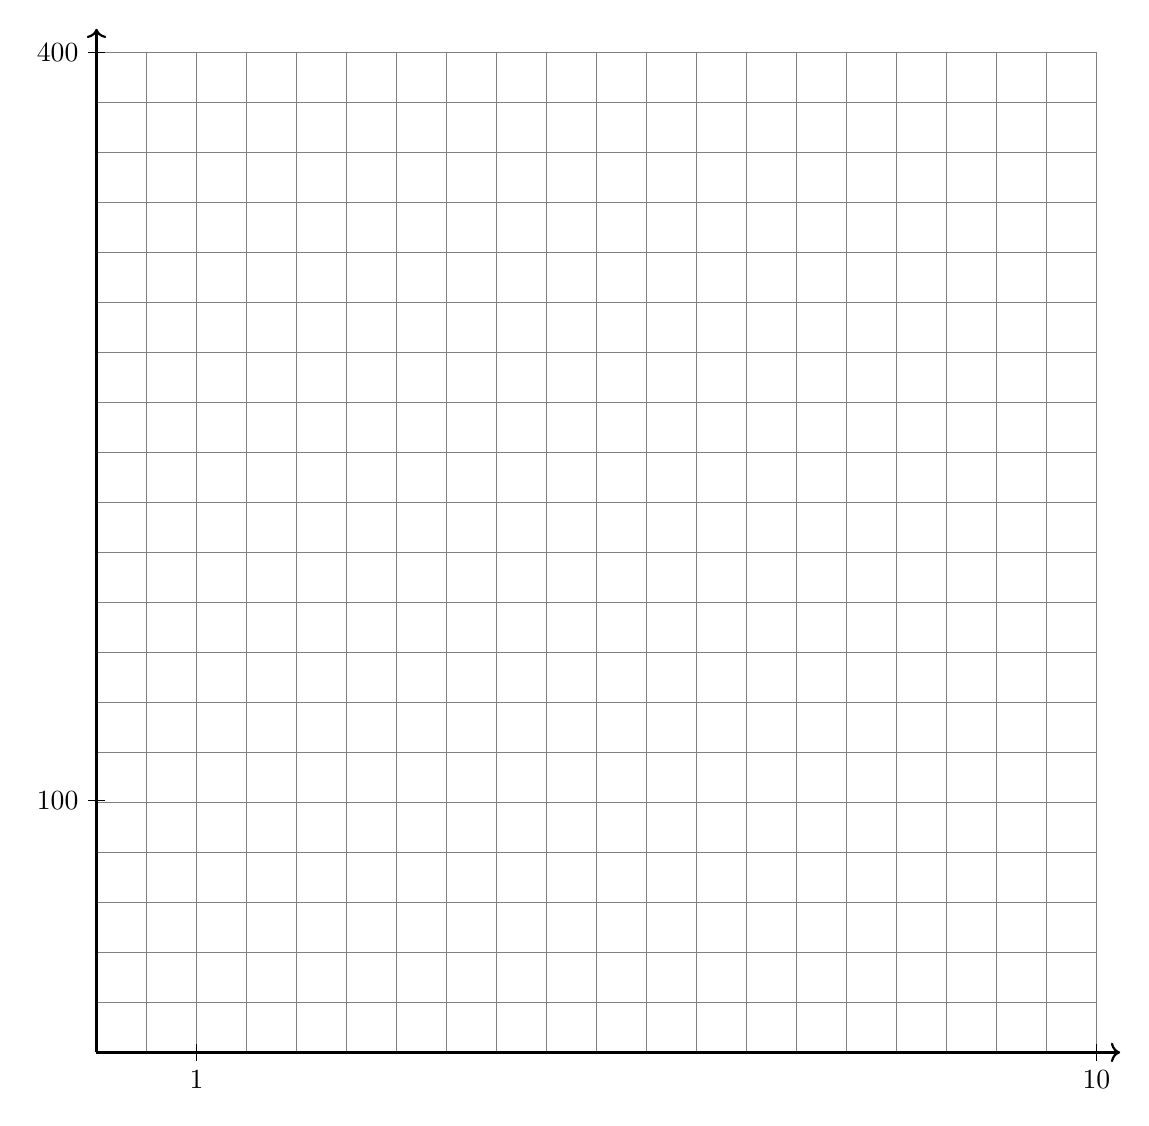
\begin{tikzpicture}
    \draw[step=0.25in,gray,very thin] (0,0) grid (12.7,12.7);
    \draw[thick,->] (0,0) -- (13,0); node[anchor=north west] {x};
    \draw[thick,->] (0,0) -- (0,13); node[anchor=south east] {y};
    \foreach \x in {1.27} \draw (\x cm,3pt) -- (\x cm,-3pt) node[anchor=north] {$1$};
    \foreach \x in {12.7} \draw (\x cm,3pt) -- (\x cm,-3pt) node[anchor=north] {10};
    \foreach \y in {3.2} \draw (3pt,\y cm) -- (-3pt,\y cm) node[anchor=east] {100};
    \foreach \y in {12.7} \draw (3pt,\y cm) -- (-3pt,\y cm) node[anchor=east] {400};
    \end{tikzpicture}
\end{center} %Alg2 Regents Jun2017

\item Use the exponent rules to rewrite the function in \#1, $f(x)$, as exponential function with only $x$ in the exponent. In other words, if $f(x)=b^x+10$, what is $b$? 


\end{enumerate}
\end{document}